\documentclass{report}
\usepackage{pdfpages}
\usepackage{graphicx} 
\usepackage{dirtytalk}
\usepackage{lmodern}
\usepackage{booktabs}
\usepackage{listings}
\usepackage{float}
\usepackage{siunitx}
\usepackage{amsmath}
\usepackage{rotating}
\usepackage{arydshln}
\usepackage[hidelinks]{hyperref}
\usepackage[ngerman]{babel}
\usepackage[a4paper, total={6in, 8in}]{geometry}
\usepackage{caption}

\newcommand{\source}[1]{\caption*{Source: {#1}} }

\begin{document}
% 
\includepdf[pages=-]{./PDFs/Deckblatt_P2}
\begin{titlepage}
    \begin{center}
        \vspace*{1cm}
            
        \Huge
        \textbf{Auswertung und Protokoll}
            
        \vspace{0.5cm}
        \LARGE
        Zum Versuch TEP
        
        \vspace{1.8cm}

        \textbf{Jonas Müther \& Alejandro Schultheiss}
        \vfill
            
        P2 Praktikum\\
       
            
        \vspace{0.8cm}
  

        \vspace{1.8cm}
        \Large
        LMU München \\
        Physik B.Sc.\\
        Deutschland\\
        2026
            
    \end{center}
\end{titlepage}
\tableofcontents

\newpage
\chapter{Vorbereitung}

\section{Versuchsvorbereitung und Grundlagen des Versuchs}
% \includepdf[pages=-]{./PDFs/TEMP_VORBEREITUNG.pdf}

\section{Versuchsprotokoll}
% \includepdf[pages=-]{./PDFs/TEMP_VERSUCHSDURCHFUEHRUNG.pdf}

\newpage
\chapter{Auswertung}
\section{Teilversuch I:Isotherme Zustandsänderung}
In den Teilversuchen I-IV wurde ein Kreisprozess untersucht. Im Ersten Teilversuch wurde eine Isotherme Expansion durchgeführt. Der Druck innerhalb der Kammer 
wurde mithilfe eines Quecksilber Manometers bestimmt. Zu diesem muss dann noch der Atmosphärendruck addiert werden.
Der Atmosphärendruck zum Versuchszeitraum wurde aus dem Internet von der Seite der Fakultät für Meteorologie der LMU München abgelesen und lag bei 
$p_{\mathrm{atm}} = \qty{961.5}{\hecto\pascal}$
Zur Umrechnung in die Einheit $\si{mmHg}$ wurde folgender Zusammenhang genutzt:
\begin{equation}
    \begin{split}
        p_{\mathrm{atm}}    &= \rho_{\mathrm{Hg}} g h \\
        \Leftrightarrow h   &= \frac{p_{\mathrm{atm}}}{\rho_{\mathrm{Hg}} g} \\
                            &= \qty{723.6}{mmHg}
    \end{split}
\end{equation}
Damit berechnen sich die Drücke innerhalb der Kammer nach:
\begin{equation}
    \begin{split}
        p = p_{\mathrm{mess}} - p_0 + p_{\mathrm{atm}}
    \end{split}
\end{equation}
Wobei $p_0$ der virtuelle Druck ist, der dadurch entsteht, dass die Skala Manometer nicht genullt ist.
Berechnet man diese Werte erhält man folgendes:
\begin{table}[H]
        \begin{center}
                \begin{tabular}{|c|c|}
                        \hline
                        Kolbenposition in $mm$ & Druck in $\mathrm{mmHg}$ \\
                        \hline
                        $72$ & $723.6 \pm 0.5$ \\
                        \hline
                        $74$ & $702.6 \pm 0.5$ \\
                        \hline
                        $76$ & $685.6 \pm 0.5$ \\
                        \hline
                        $78$ & $665.6 \pm 0.5$ \\
                        \hline
                        $80$ & $651.6 \pm 0.5$ \\
                        \hline
                        $82$ & $635.6 \pm 0.5$ \\
                        \hline
                        $84$ & $619.6 \pm 0.5$ \\
                        \hline
                        $86$ & $607.6 \pm 0.5$ \\
                        \hline
                        $88$ & $594.6 \pm 0.5$ \\
                        \hline
                        $90$ & $581.6 \pm 0.5$ \\
                        \hline
                \end{tabular}
        \end{center}
        \caption{Gemessene Drücke in mmHg}
        \label{tab:IsoThermExpPmmHg}
\end{table}
Mithilfe dieser Werte wollen wir das Boyle-Mariottesche Gesetz bestätigen.
Dieses besagt:
\begin{equation}
    \begin{split}
        pV &= const \\
        \Leftrightarrow pV &= p_0 V_0 \\
        \Leftrightarrow \frac{p_0}{p} &= \frac{V}{V_0} \\
        \Leftrightarrow \frac{p_0}{p} &= \frac{x}{x_0}
    \end{split}
\end{equation}
Das Gesetz ist also bestätigt, falls das $\frac{p_0}{p}(x)$-Diagramm eine Gerade mit der Steigung $\frac{1}{x_0}$ ergibt.
Um dies zu prüfen plotten wir dieses Diagramm und legen eine Ausgleichsgerade. Aus der Steigung der Ausgleichsgerade berechnen wir dann $x_0^{\mathrm{steig}} = 1/m$
\begin{figure}[H]
    \centering
    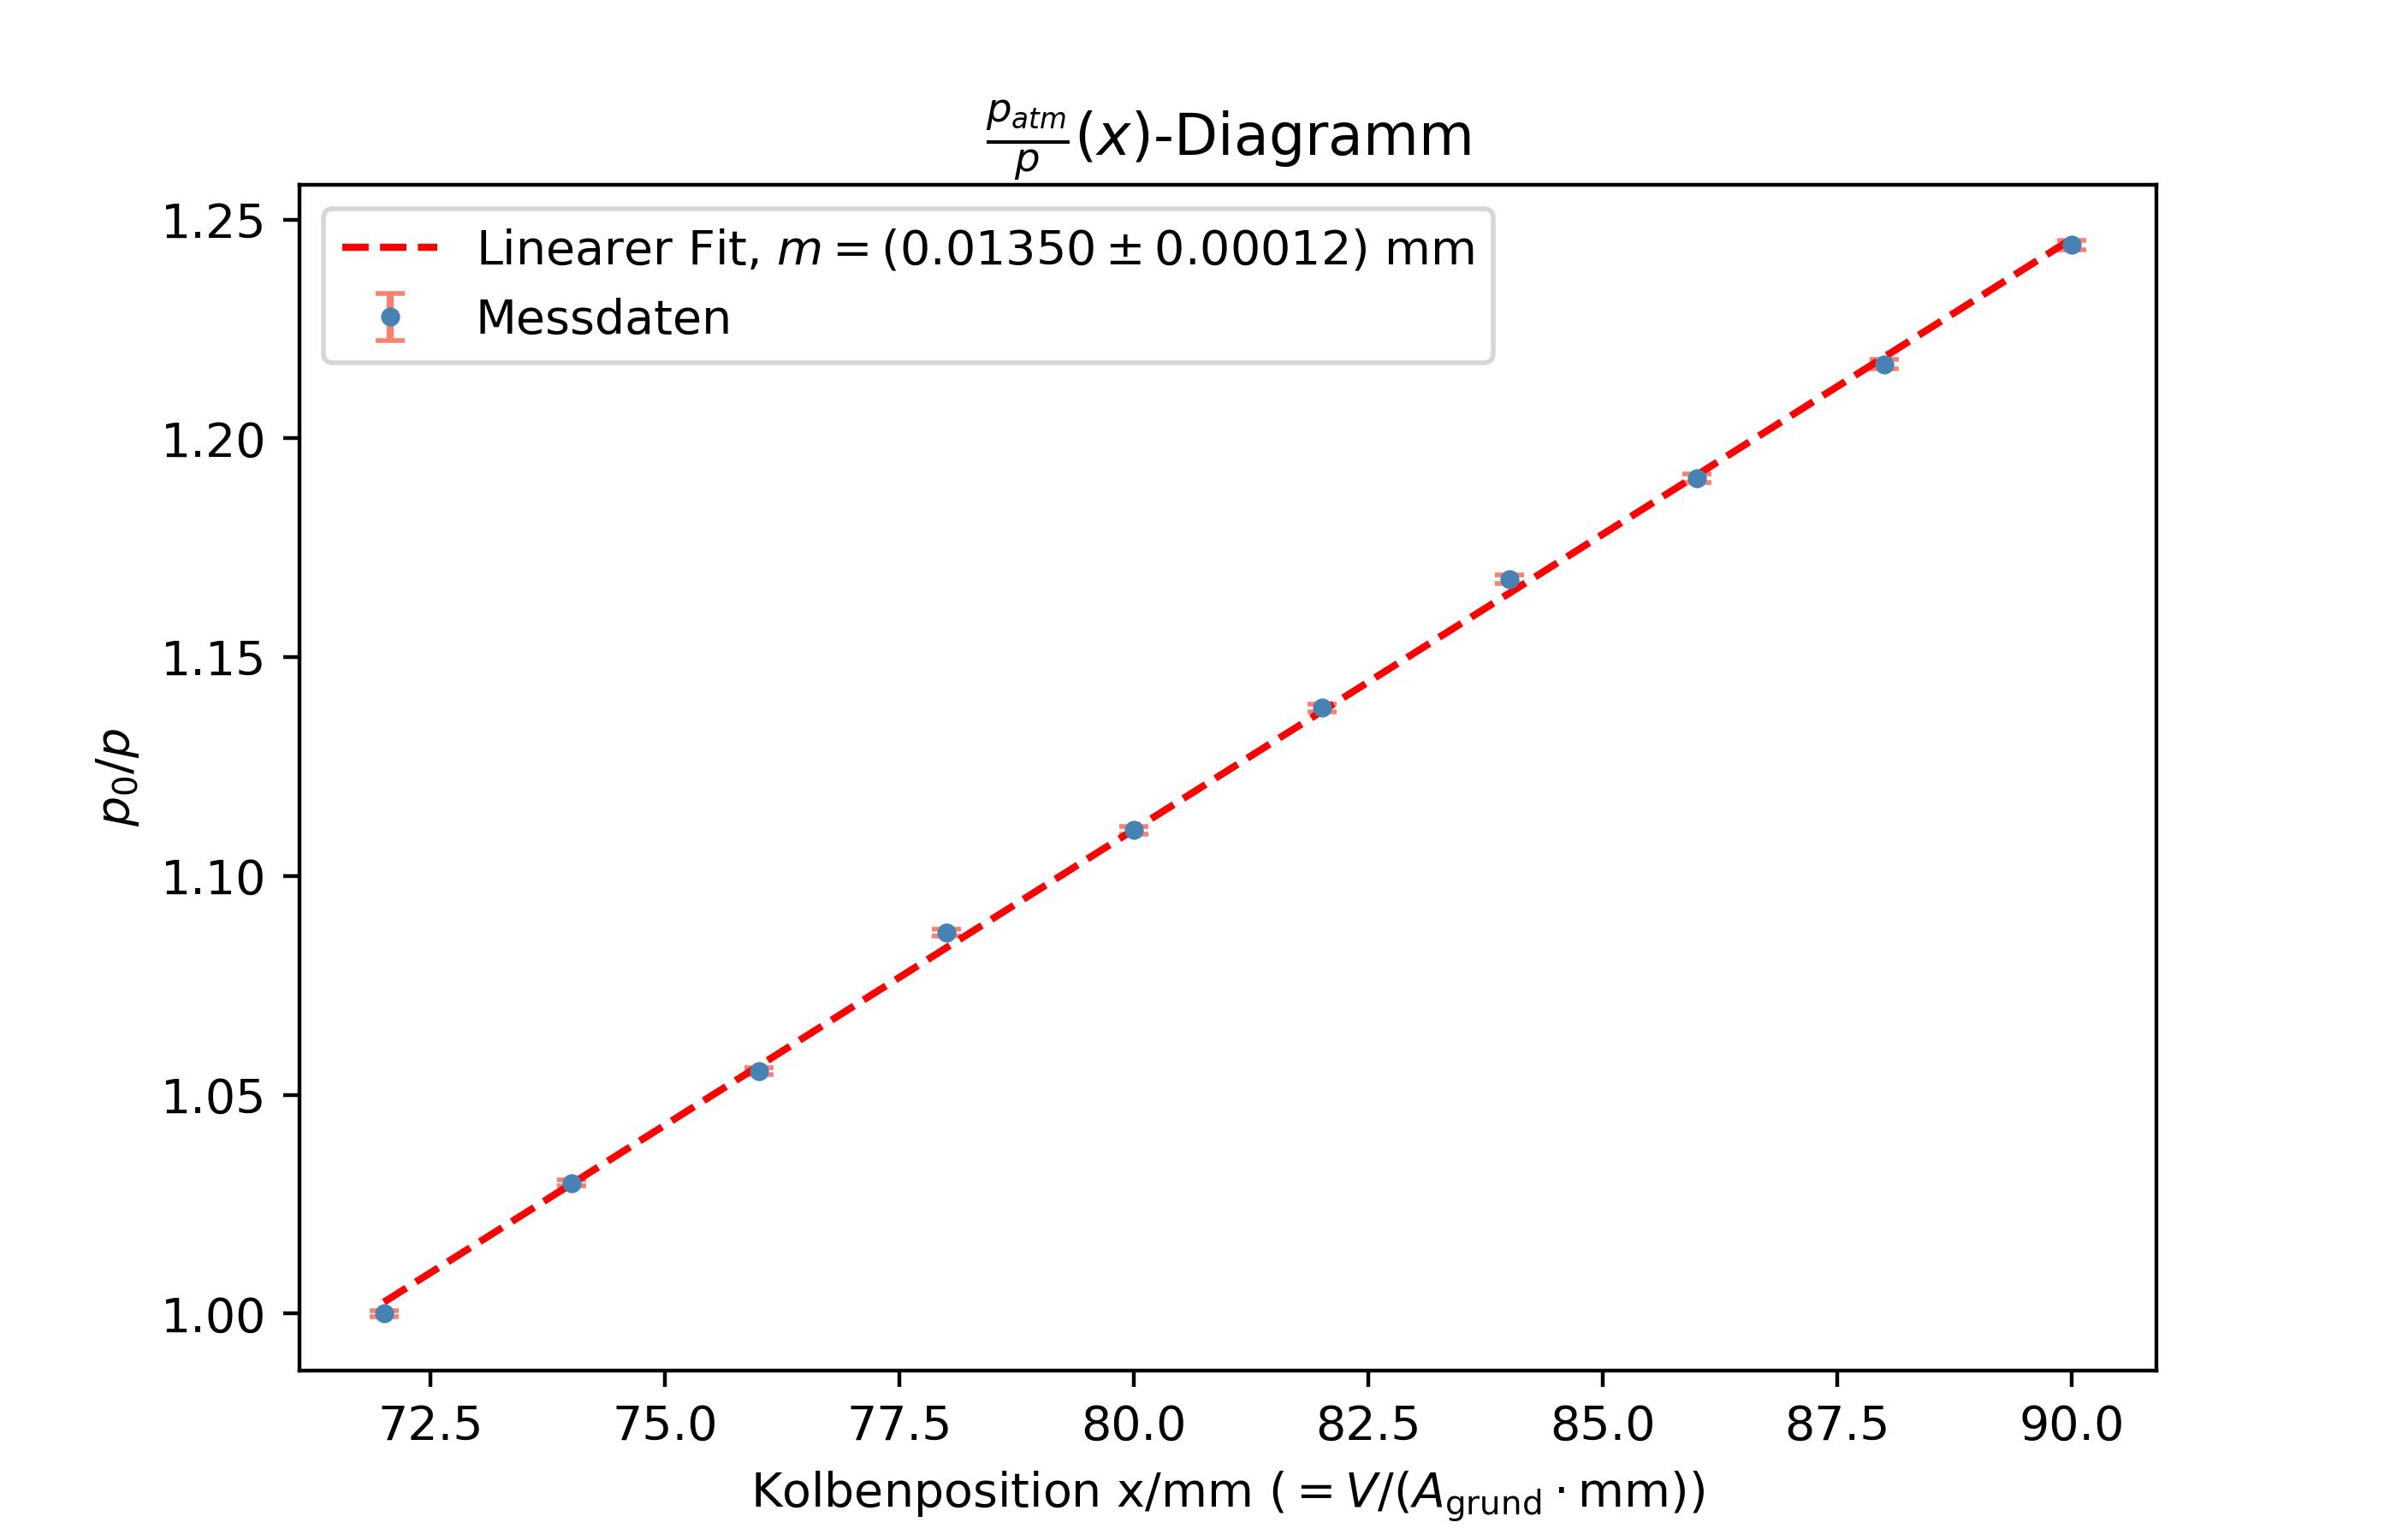
\includegraphics[width=1\textwidth]{./Images/TV1_DiagrammP0-P-x-Diagramm.jpg}
    \caption{$\frac{p_0}{p}(x)$-Diagramm}
    \label{fig:IsoThermExpP0/P-x-Diagramm}
\end{figure}
\noindent
Tatsächlich liegen die Werte relativ gut auf einer Geraden. Berechnet man nun aus deren Steigung den Wert $x_0^{\mathrm{steig}}$:
\begin{equation}
    \begin{split}
        x_0^{\mathrm{steig}} = \qty{74.1}{mm}
    \end{split}
\end{equation}
Dieser Wert stimmt ungefähr mit dem tatsächlichen Wert $x_0 = \qty{72.0}{mm}$ überein. Dennoch gibt es eine geringe Abweichung. Diese könnte beispielsweise auf die Fehler 
beim Ablesen der Quecksilbersäule und beim Einstellen der Drücke zurückzuführen sein.

\section{Teilversuch II: Isochore Zustandsänderung}
In Teilversuch II wurde die Temperatur im Kolben bei konstanter Kolbenposition (gleichem Volumen) langsam verringert. Die hierbei auftretende isochore Zustandsänderung 
soll im folgenden untersucht werden. 
Für eine isochore Zustandsänderung gilt das folgende empirisch Gefundene Gesetz von Amontons:
\begin{equation}
    p = p_0(1+\beta \theta)
    \label{eq:Amontons}
\end{equation}
Für eine ideales Gas liegt der Isochore Spannungskoeffizient bei:
\begin{equation}
    \beta = \frac{1}{T_0}
\end{equation}
Die im Versuch verwendete Luft wird im folgenden als ideales Gas angenommen.
Folgende Wert wurden während der Temperaturerniedrigung gemessen:
\begin{table}[H]
        \begin{center}
                \begin{tabular}{|c|c|}
                        \hline
                        Temperatur in °C & Druck in $\mathrm{mmHg}$ \\
                        \hline
                        $89.30 \pm 0.13$ & $581.6 \pm 0.5$ \\
                        \hline
                        $74.80 \pm 0.13$ & $559.6 \pm 0.5$ \\
                        \hline
                        $59.00 \pm 0.12$ & $534.6 \pm 0.5$ \\
                        \hline
                        $44.90 \pm 0.12$ & $510.6 \pm 0.5$ \\
                        \hline
                        $29.70 \pm 0.11$ & $487.6 \pm 0.5$ \\
                        \hline
                        $14.80 \pm 0.11$ & $454.6 \pm 0.5$ \\
                        \hline
                        $0.50 \pm 0.11$ & $427.6 \pm 0.5$ \\
                        \hline
                \end{tabular}
        \end{center}
        \caption{Gemessene Drücke bei verschiedenen Temperaturen in mmHg}
        \label{tab:IsochorPmmHg}
\end{table}
Plottet man diese Messwerte und legt eine Ausgleichsgerade hindurch, erhält man folgenden Graphen:
\begin{figure}[H]
    \centering
    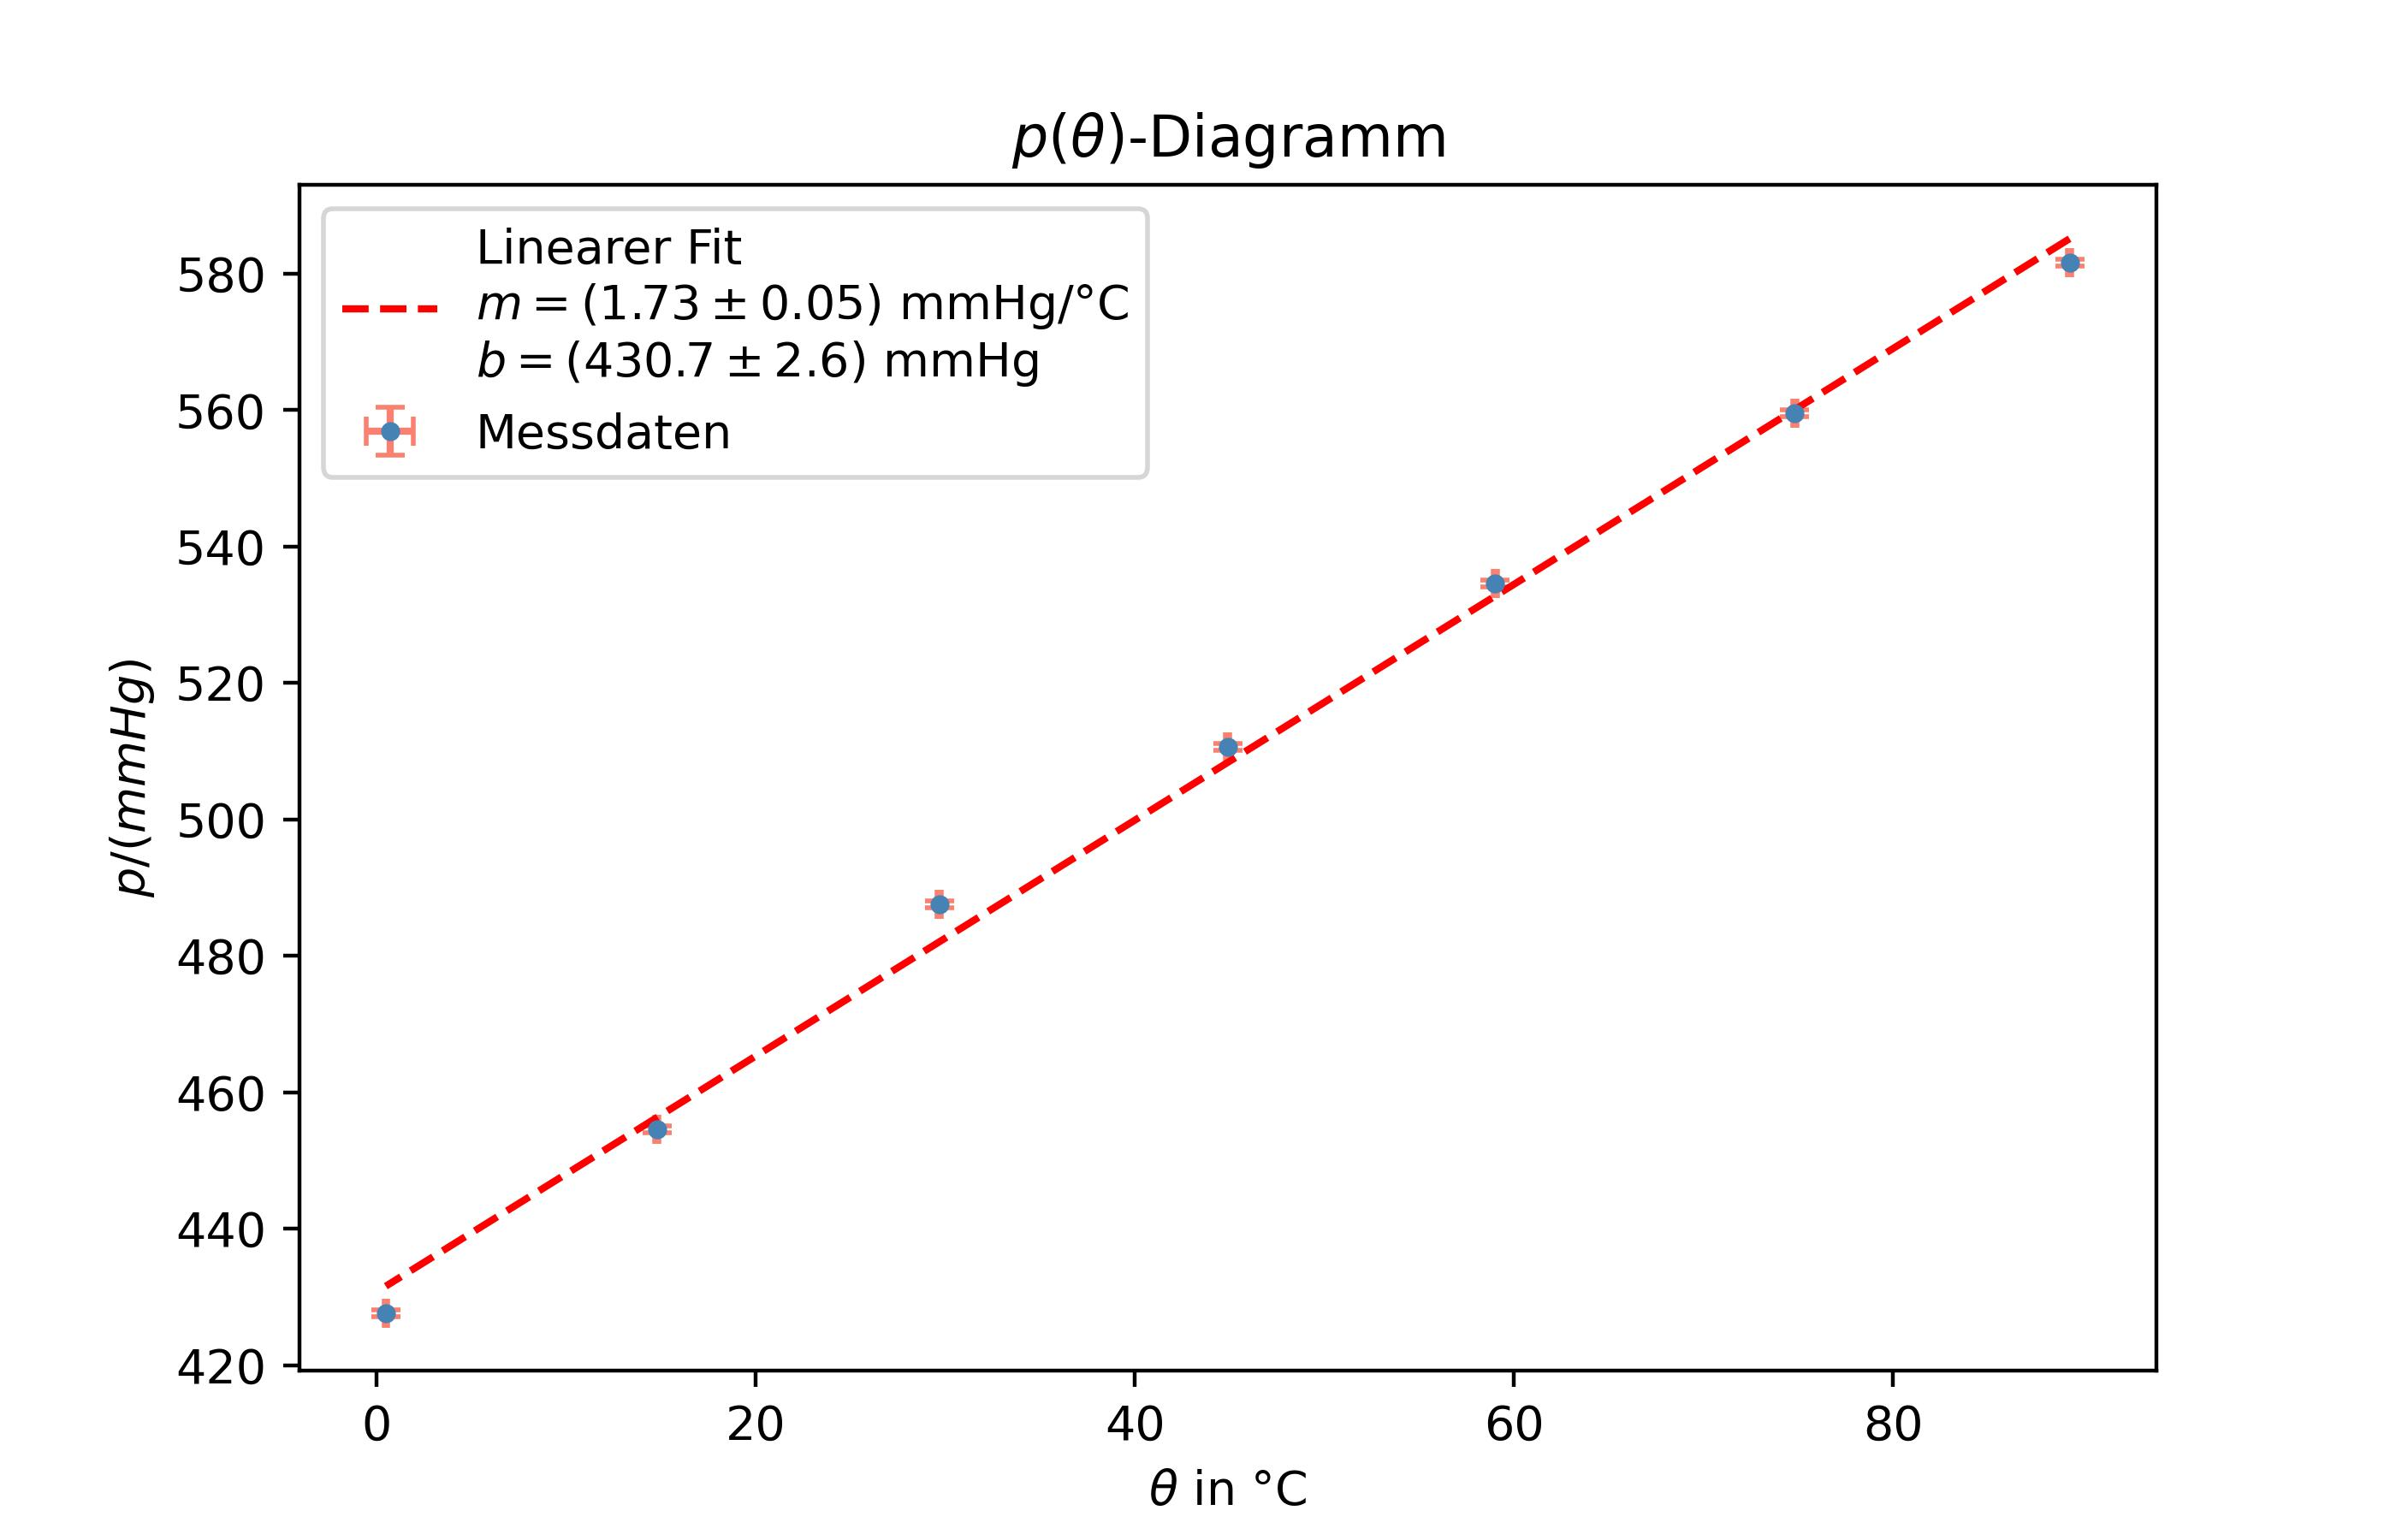
\includegraphics[width=1\textwidth]{./Images/TV2_P-T-Diagramm.jpg}
    \caption{$p(\theta)$-Diagramm einer Isochoren Temperaturerhöhung}
    \label{fig:P-T-Diagramm}
\end{figure}
Es ist gut erkennbar, dass die Messwerte in sehr guter Näherung auf der Ausgleichsgeraden liegen. Der Temperaturabhängige Druck kann also
näherungsweise durch die Ausgleichsgerade angegeben werden:
\begin{equation}
    \begin{split}
        p = m\theta + b
    \end{split}
\end{equation}
Durch Gleichsetzen mit Gleichung \ref{eq:Amontons} und Koeffizientenvergleich kann damit $\beta$ berechnet werden:
\begin{equation}
    \begin{split}
        m\theta + b &= p_0(1+\beta\theta) \; \; \forall \theta \\
        \Leftrightarrow \beta &= \frac{m}{b} \\
        \Leftrightarrow T_0 &= \frac{b}{m}
    \end{split}
\end{equation}
Durch Einsetzen der Werte erhält man für den isochoren Spannungskoeffizient:
\begin{equation}
    \beta = \qty{4.017e-3}{\per\kelvin}
\end{equation}
Für $T_0$ kommt man auf:
\begin{equation}
    T_0 = \qty{249.0}{\kelvin}
\end{equation}
Dieser Wert liegt relativ weit entfernt vom Literaturwerwt von $T_0^{\mathrm{lit}} = 273.15K$. Hierfür kann es verschiedene Gründe geben.
Einerseits handelt es sich beim Atmosphärendruck aus dem Internet um einen Wert, der nicht direkt vor Ort gemessen wurde. Dieser geht bei der Umrechnung des 
Manometerwerts in einen absoluten Wert ein und hat so Einfluss auf das Endergebnis. Außerdem spielt auch hier die Ungenauigkeit beim Einstellen des Spiegels des 
Manometers eine Entscheidende Rolle. Zudem handelt es sich bei Luft nicht um ein perfektes ideales Gas, was zu einer (wenn auch relativ kleinen) Abweichung führt. 
Der möglicherweise wichtigste Faktor, der zur großen Abweichung beiträgt ist allerdings die ungleiche Temperaturverteilung im System. Da die Temperatur während des Versuchs 
durch die Eiszugabe schnell gesunken ist, ist es gut möglich, dass die Temperatur der Luft in der Kammer noch signifikant oberhalb der Temperatur des Wassers bzw. des Termometers 
lag. Dies ist auf die nur endliche Wärmeleitfähigkeit der Metallkammer und auf die schlechte Wärmeleitfähigkeit in der Luft zurückzuführen.

\newpage
\section{Teilversuch III: }

\newpage
\section{Teilversuch IV: }

\newpage
\section{Teilversuch V: }
\noindent
In diesem Teilversuch wurde der Adiabatenexponent $\gamma$ von Luft mithilfe
einer schwingenden Wassersäule bestimmt. Die Schwingungsdauer wurde jeweils
ohne und mit angeschlossenem Glaskolben gemessen. Nach der Versuchsanleitung gilt

\begin{equation}
\gamma=
\frac{2\rho gV}{p_0A}
\left(
\frac{\tau_0^2}{\tau_k^2}-1
\right),
\label{eq:gamma}
\end{equation}
\noindent
wobei $\tau_0$ die Periodendauer ohne Kolben und $\tau_k$ diejenige mit
Kolben bezeichnet.


\subsubsection{Bestimmung der Periodendauern}
\noindent
Gemessen wurde jeweils die Zeit für fünf Schwingungen. Die Messreihen lauten

\begin{table}[htbp]
    \centering
    \caption{Gemessene Zeiten für jeweils fünf Schwingungen.}
    \begin{tabular}{c|c|c}
        \hline
        Messung & $t_0$ ohne Kolben in $\mathrm{s}$
                & $t_k$ mit Kolben in $\mathrm{s}$\\
        \hline
        1 & 5{,}21 & 3{,}41\\
        2 & 5{,}05 & 3{,}72\\
        3 & 5{,}19 & 3{,}50\\
        4 & 5{,}22 & 3{,}37\\
        5 & 5{,}22 & 3{,}56\\
        \hline
    \end{tabular}
\end{table}
\noindent
Für die Mittelwerte für fünf Schwingungen gilt:

\begin{equation}
\overline{t}_0=5{,}178\,\mathrm{s},
\qquad
\overline{t}_k=3{,}512\,\mathrm{s}.
\end{equation}
\noindent
Damit folgen die mittleren Periodendauern

\begin{equation}
\overline{\tau}_0=1{,}0356\,\mathrm{s},
\qquad
\overline{\tau}_k=0{,}7024\,\mathrm{s}.
\end{equation}
\noindent
Zur Berücksichtigung der statistischen Streuung wurde zunächst die empirische
Standardabweichung

\begin{equation}
s_\tau=
\sqrt{\frac{1}{n-1}
\sum_{i=1}^{n}(\tau_i-\overline{\tau})^2}
\end{equation}
\noindent
und daraus die Standardabweichung des Mittelwertes

\begin{equation}
s_{\overline{\tau}}=\frac{s_\tau}{\sqrt{n}}
\end{equation}
\noindent
berechnet. Es ergeben sich

\begin{align}
s_{\tau_0}&=0{,}01452\,\mathrm{s},
&
s_{\overline{\tau}_0}&=0{,}00649\,\mathrm{s},\\
s_{\tau_k}&=0{,}02762\,\mathrm{s},
&
s_{\overline{\tau}_k}&=0{,}01235\,\mathrm{s}.
\end{align}
\noindent
Damit werden für die weitere Auswertung

\begin{equation}
\boxed{\tau_0=(1{,}036\pm0{,}007)\,\mathrm{s}}
\end{equation}
\noindent
und

\begin{equation}
\boxed{\tau_k=(0{,}702\pm0{,}013)\,\mathrm{s}}
\end{equation}
\noindent
verwendet.


\subsubsection{Bestimmung des eingeschlossenen Luftvolumens}
\noindent
Das Volumen des Glaskolbens wurde durch Wägung ohne und mit Wasser bestimmt:

\begin{equation}
m_\mathrm{leer}=(254{,}41\pm0{,}03)\,\mathrm{g},
\qquad
m_\mathrm{voll}=(1370{,}90\pm0{,}03)\,\mathrm{g}.
\end{equation}

Mit $\rho_\mathrm{W}=1{,}00\,\mathrm{g/cm^3}$ folgt

\begin{equation}
V_\mathrm{K}
=
\frac{m_\mathrm{voll}-m_\mathrm{leer}}{\rho_\mathrm{W}}
=
1116{,}49\,\mathrm{cm^3}.
\end{equation}
\noindent
Für den Innendurchmesser und die Höhe der zusätzlichen Luftsäule wurden

\begin{equation}
d=(1{,}8\pm0{,}1)\,\mathrm{cm},
\qquad
h=(23{,}6\pm0{,}1)\,\mathrm{cm}
\end{equation}
\noindent
gemessen. Der Rohrquerschnitt beträgt damit

\begin{equation}
A=\frac{\pi d^2}{4}
=
2{,}54469\,\mathrm{cm^2}.
\end{equation}
\noindent
Für das zusätzliche Luftvolumen ergibt sich

\begin{equation}
V_\mathrm{R}=Ah
=
60{,}05\,\mathrm{cm^3}.
\end{equation}
\noindent
Damit beträgt das gesamte eingeschlossene Luftvolumen

\begin{equation}
\boxed{
V=V_\mathrm{K}+V_\mathrm{R}
=
1176{,}54\,\mathrm{cm^3}
=
1{,}17654\cdot10^{-3}\,\mathrm{m^3}
}.
\end{equation}
\noindent
Der Atmosphärendruck am Versuchstag betrug (gemäß Institut für Meteorologie LMU München abgerufen via. Internet-Browser)

\begin{equation}
p_0=961{,}5\,\mathrm{hPa}
=96150\,\mathrm{Pa}.
\end{equation}
\noindent
Da auf der Seite der LMU bzgl. Luftdruck in München keine Unsicherheit angegeben wurde, wird entsprechend der angegebenen
Auflösung für die Unsicherheitsrechnung

\begin{equation}
\Delta p_0=0{,}1\,\mathrm{hPa}=10\,\mathrm{Pa}
\end{equation}
\noindent
angesetzt.


\subsubsection{Berechnung des Adiabatenexponenten}

Mit $\rho=1000\,\mathrm{kg/m^3}$ und
$g=9{,}81\,\mathrm{m/s^2}$ ergibt sich zunächst

\begin{equation}
\frac{\tau_0^2}{\tau_k^2}-1
=
1{,}17378.
\end{equation}
\noindent
Einsetzen in Gleichung~\ref{eq:gamma} liefert

\begin{align}
\gamma
&=
\frac{
2\cdot1000\cdot9{,}81
\cdot1{,}17654\cdot10^{-3}
}{
96150\cdot2{,}54469\cdot10^{-4}
}
\left(
\frac{1{,}0356^2}{0{,}7024^2}-1
\right)\\
&=
1{,}1074.
\end{align}


\subsubsection{Gaußsche Fehlerfortpflanzung}
\noindent
Die Gesamtunsicherheit wird mit

\begin{equation}
\Delta\gamma
=
\sqrt{
\sum_i
\left(
\frac{\partial\gamma}{\partial x_i}
\Delta x_i
\right)^2
}
\end{equation}
\noindent
bestimmt.
\noindent
Dabei wurde berücksichtigt, dass die Querschnittsfläche $A$ und der Rohranteil
des Volumens $V$ beide vom Durchmesser $d$ abhängen. Daher wurde die
Fehlerfortpflanzung direkt über die unabhängig gemessenen Größen
$m_\mathrm{voll}$, $m_\mathrm{leer}$, $h$, $d$, $\tau_0$, $\tau_k$ und $p_0$
durchgeführt.
\noindent
Die einzelnen Beiträge sind in Tabelle~\ref{tab:budget_gamma} angegeben.

\begin{table}[htbp]
    \centering
    \caption{Messunsicherheitsbudget für $\gamma$.}
    \label{tab:budget_gamma}
    \begin{tabular}{c|c}
        \hline
        Eingangsgröße & Beitrag zu $\Delta\gamma$\\
        \hline
        $m_\mathrm{voll}$ & $2{,}8\cdot10^{-5}$\\
        $m_\mathrm{leer}$ & $2{,}8\cdot10^{-5}$\\
        $h$               & $2{,}4\cdot10^{-4}$\\
        $d$               & $0{,}1168$\\
        $\tau_0$          & $0{,}0257$\\
        $\tau_k$          & $0{,}0721$\\
        $p_0$             & $1{,}2\cdot10^{-4}$\\
        \hline
    \end{tabular}
\end{table}
\noindent
Durch quadratische Addition ergibt sich

\begin{equation}
\Delta\gamma
=
0{,}1396\ldots
\end{equation}
\noindent
und damit gerundet

\begin{equation}
\boxed{
\gamma_\mathrm{exp}=1{,}11\pm0{,}14
}.
\end{equation}
\noindent
Die Gesamtunsicherheit wird deutlich von der Messung des Rohrdurchmessers
dominiert. Ursache hierfür ist, dass der Durchmesser quadratisch in

\begin{equation}
A=\frac{\pi d^2}{4}
\end{equation}
\noindent
eingeht. Der zweitgrößte Beitrag stammt aus der statistischen Unsicherheit der
Periodendauer $\tau_k$.


\subsubsection{Vergleich und Diskussion}
\noindent
Für Luft wird bei Raumtemperatur theoretisch ein Adiabatenexponent von

\begin{equation}
\gamma_\mathrm{theo}
=
\frac{7}{5}
=
1{,}4
\end{equation}
\noindent
erwartet.
\noindent
Experimentell wurde

\begin{equation}
\boxed{
\gamma_\mathrm{exp}
=
1{,}11\pm0{,}14
}
\end{equation}
\noindent
bestimmt. Die relative Abweichung des Zentralwertes vom theoretischen Wert beträgt

\begin{equation}
\delta
=
\frac{
|\gamma_\mathrm{exp}-\gamma_\mathrm{theo}|
}{
\gamma_\mathrm{theo}
}
\cdot100\,\%
\approx
20{,}9\,\%.
\end{equation}
\noindent
Der theoretische Wert liegt damit nicht innerhalb des einfachen
Unsicherheitsintervalls des experimentellen Ergebnisses. Die Abweichung kann
folglich nicht allein durch die berücksichtigten statistischen und direkt
quantifizierten Messunsicherheiten erklärt werden.
\noindent
Ein wesentlicher Beitrag zur Unsicherheit entsteht durch die Bestimmung des
Innendurchmessers des U-Rohrs. Da der Durchmesser quadratisch in die
Querschnittsfläche

\begin{equation}
A=\frac{\pi d^2}{4}
\end{equation}
\noindent
eingeht, wirkt sich bereits eine vergleichsweise kleine Unsicherheit von $d$
deutlich auf das Ergebnis für $\gamma$ aus. In dem erstellten
Messunsicherheitsbudget ist dieser Beitrag entsprechend dominant.
\noindent
Zusätzlich treten systematische Einflüsse auf, die durch die Gaußsche
Fehlerfortpflanzung nur unvollständig erfasst werden. Die Zustandsänderung ist
nur dann näherungsweise adiabatisch, wenn die Kompression und Expansion der
eingeschlossenen Luft hinreichend schnell abläuft. Ein Wärmeaustausch mit den
Glaswänden und der Umgebung kann daher dazu führen, dass der reale Prozess vom
idealen adiabatischen Verhalten abweicht.
\noindent
Weiterhin setzt die verwendete Näherung insbesondere bei angeschlossenem Kolben
eine kleine Schwingungsamplitude voraus. Wird diese Bedingung nicht vollständig
eingehalten, kann die zugrunde gelegte lineare Beziehung zwischen Druck- und
Volumenänderung verletzt sein.
\noindent
Weitere mögliche systematische Fehlerquellen sind ein nicht exakt bekannter
effektiver Rohrquerschnitt, zusätzliche kleine Verbindungsvolumina sowie die
manuelle Zeitmessung. Insbesondere die Messreihe mit angeschlossenem Kolben zeigt
eine vergleichsweise große Streuung der Schwingungszeiten.
\noindent
Insgesamt stimmt der experimentelle Wert daher nicht quantitativ mit dem
theoretischen Wert überein. Die beobachtete Abweichung ist jedoch angesichts der
experimentellen Randbedingungen und der vorhandenen systematischen
Unsicherheiten plausibel. Das Ergebnis ist somit mit der theoretischen
Größenordnung vereinbar, stellt aber keine präzise Bestätigung des
Literaturwertes dar.








\newpage
\chapter{Anhang}
\section{Python Scripts}
Die Python Scripts, die zum Plotten der Grafiken verwendet wurden, wurden mit Unterstützung von KI erstellt und dann nach den eigenen Bedürfnissen weiter
bearbeitet.
\definecolor{codegreen}{rgb}{0,0.6,0}
\definecolor{codegray}{rgb}{0.5,0.5,0.5}
\definecolor{codepurple}{rgb}{0.58,0,0.82}
\definecolor{backcolour}{rgb}{0.95,0.95,0.92}

\lstdefinestyle{python}{
    backgroundcolor=\color{backcolour},   
    commentstyle=\color{codegreen},
    keywordstyle=\color{magenta},
    numberstyle=\tiny\color{codegray},
    stringstyle=\color{codepurple},
    basicstyle=\ttfamily\footnotesize,
    breakatwhitespace=false,         
    breaklines=true,                 
    captionpos=b,                    
    keepspaces=true,                 
    numbers=left,                    
    numbersep=5pt,                  
    showspaces=false,                
    showstringspaces=false,
    showtabs=false,                  
    tabsize=2
}

\end{document}
